%! TeX program = lualatex
\documentclass[12pt,a4paper]{instrukcja}

\begin{document}

\thispagestyle{empty}

\begin{center}
	\vspace*{2cm}

	\header{{\Huge Wybrane celebracje w Roku Liturgicznym}\\\bigskip{\large wg
			Mszału 1962}}

	\vspace{\fill}

	{\large \textbf{Użyte oznaczenia:}} \\

	\vspace{0.05\textwidth}

	{\large
		\begin{table}[!h]
			\large
			\hspace{6cm}
			\begin{tabular}{r c l}
				\ii                  & -- & celebrans           \smallskip \\
				\dd                  & -- & diakon              \smallskip \\
				\ss                  & -- & subdiakon           \smallskip \\
				\cc                  & -- & ceremoniarz         \smallskip \\
				\aa                  & -- & akolita             \smallskip \\
				\tt                  & -- & turyfer             \smallskip \\
				\ding{63}            & -- & krzyż procesyjny    \smallskip \\
				\oo                  & -- & ombrelino           \smallskip \\
				\zz                  & -- & zakrystianin        \smallskip \\
				\bb                  & -- & ministrant księgi   \smallskip \\
				\spiew~ \eighthnote~ & -- & śpiewający          \smallskip \\
				\kolatki             & -- & kołatki             \smallskip \\
				\paschal             & -- & ministrant Paschału \smallskip \\
			\end{tabular}
		\end{table}
	}

	\vspace{0.5cm}

	\begin{figure}[!htbp]
		\centering
		
\includegraphics[width=0.3\linewidth]{Figures/logo.png}
	\end{figure}

	\footer{Autorzy: Jakub Gajewski, Marek Skarupski, Piotr Matuszak, Michał Siemaszko, Maciej Rumin i inni}
\end{center}



\thispagestyle{empty}

\tableofcontents

% \newpage

\pagestyle{plain}

\chapter{Oczyszczenie NMP}

\section{Poświęcenie Gromnic i procesja}

\begin{itemize}
	\item Do prezbiterium wychodzimy normalnie, kapłan ubrany w białą kapę
	\item Po \textit{Dominus vobiscum} następuje 5 oracji po czym zasypanie,
	      pokropienie i okadzenie (potrzebny turyfer i ministrant z kropielnicą)
	      \footnote{\textbf{UWAGA}: może być tak, że celebrans pójdzie pokropić
		      świece wiernych}
	\item Świece rozdawane są ministrantom w sposób podobny do przyjmowania
	      Komunii Św.
	      \footnote{w trakcie rozdawania śpiewa się \textit{Pieśń Symeona}}
	\item Po zakończeniu rozdawania świec następuje ostatnia oracja
	\item Formuje się procesja z krzyżem i akolitami. Idą w niej wszyscy
	      ministranci, celebrans oraz  wierni. Wszyscy mają \underline{zapalone świece}.
	\item Idziemy dookoła kościoła i wracamy do prezbiterium
	\item Po powrocie celebrans zakłada biały ornat i wszyscy gaszą gromnice
\end{itemize}

\section{Zmiany na Mszy Świętej}

\begin{itemize}
	\item Brak modlitw u stopni ołtarza
	\item Msza z dnia bez perturbacji
	\item Zapalamy gromnice na Ewangelię i od \textit{Sanctus} do końca Kanonu.
	\item Zaleca się zrobienie lucenarium
\end{itemize}


\chapter{Pasterka}

\section{Procesja wejścia}

\begin{itemize}
	\item W kościele należy wygasić światła.
	\item Kapłan ubrany w kapę koloru białego bez akompaniamentu organów
	      się do żłóbka ustawionego w prezbiterium. (W tym czasie jeden z
	      usługujących może uderzyć 12 razy w gong)
	\item Po przyjściu kładzie figurkę Dzieciątka i przykrywa ją welonem.
	      Następnie staje przy krześle wraz z asystą.
	\item Kantor staje na ambonie i śpiewa Kalendę: \smallbreak
	      %
	      \inde{Octavo Kalendas Januarii Luna N.\\
		      Innumeris transactis saeculis a creatione mundi, quando in
		      principio Deus creavit caelum et terram et hominem formavit ad
		      imaginem suam;\\
		      permultis etiam saeculis, ex quo post diluvium Altissimus in
		      nubibus arcum posuerat, signum fœderis et pacis;\\
		      a migratione Abrahæ, patris nostri in fide, de Ur Chaldæorum
		      saeculo vigesimo primo;\\
		      ab egressu populi Israël de Ægypto, Moyse duce, saeculo decimo
		      tertio;\\
		      ab unctione David in regem, anno circiter millesimo;\\
		      hebdomada sexagesima quinta, juxta Danielis prophetiam;\\
		      Olympiade centesima nonagesima quarta;\\
		      ab Urbe condita anno septingentesimo quinquagesimo secundo;\\
		      anno imperii Cæsaris Octaviani Augusti quadragesimo secundo;\\
		      toto orbe in pace composito, \textbf{Jesus Christus}, æternus Deus
		      æternique Patris Filius, mundum volens adventu suo piissimo
		      consecrare, de Spiritu Sancto conceptus, novemque post
		      conceptionem decursis mensibus, in Bethlehem Judæ \textbf{nascitur
		      ex Maria Virgine factus homo}:}
	      \smallbreak
	\item[] Tu zapala się światła w kościele.
	      \smallbreak
	      \inde{Nativitas Domini nostri \textbf{Jesu Christi} secundum carnem.}
	      %
	\item Tu bije się we wszystkie dzwonki (podobnie jak w czasie
	      \textit{Gloria} w trakcie Wigilii Paschalnej) i odzywają się organy.
	\item Rozpoczyna się śpiew pieśni Wśród Nocnej Ciszy. Kapłan w tym czasie
	      odkrywa figurkę Dzieciątka, nakłada kadzidło do kadzielnicy i okadza
	      figurkę Dzieciątka. Można też teraz przyozdobić żłóbek kwiatami.
	\item Po zakończeniu śpiewu wszyscy siadają, a kapłan udaje się na ambonę i
	      wygłasza homilię.
	\item Po homilii kapłan ubiera szaty mszalne koloru białego i rozpoczyna
	      Mszę jak zwykle.
\end{itemize}

\section{Zmiany na Mszy Świętej}

\begin{itemize}
	\item Podczas lekcji imię \textbf{Jezus} pada dwa razy -- na oba razy
	      skłaniamy głowę w stronę krzyża
	\item Jeśli wystarczy ministrantów to robimy lucenarium
	\item Jest bożonarodzeniowe \textit{Communicantes}
\end{itemize}


% \footer{
% 	Nihil Obstat	-- Karol Pyziołek 			\hfill 
% 	Imprimatur 		-- ks. Ireneusz Bakalarczyk \hfill 
% 	Skład 			-- Michał Siemaszko}


\chapter{Popielec}

\begin{paracol}{2}
	\section{Przygotowanie do obrzędów -- msza śpiewana}

	\subsection{Na ołtarzu}

	\begin{itemize*}
		\item Mszał otwarty na obrzędy poświęcenia popiołu po stronie epistoły i
		ustawiony równolegle do krawędzi
		\item Tablice ołtarzowe na ich właściwych miejscach
		\item Tacki z popiołem do poświęcenia na stoliku z boku ołtarza lub na
		ołtarzu po stronie epistoły
		\item (Kielich ustawiony na rozłożonym korporale, bursa postawiona
		      pionowo po lewej od kielicha, tuż przy dalszej krawędzi obrusu)
		\item Sześć zapalonych świec
		\item Brak dekoracji i kwiatów
	\end{itemize*}

	\subsection{Na kredensji}

	\begin{itemize*}
		\item Woda święcona w kociołku i aspergil
		\item Miska
		\item Dzbanek z wodą
		\item Mydło
		\item Ręcznik
		\item Ampułki z wodą i winem
		\item Lawaterz
		\item Patena
		\item Dzwonki
		\item (Kielich okryty welonem naramiennym)
		\item Lekcjonarz
		\item Świeca sanctusowa
		\item Kartki do modlitw u stopni ołtarza
	\end{itemize*}

	\subsection{Na Sedilli}

	\begin{itemize*}
		\item {\color{violet}{Fioletowy ornat}}
		\item {\color{violet}{Manipularz}}
	\end{itemize*}

	\subsection{W zakrystii}

	\begin{itemize*}
		\item {\color{violet} Fioletowa kapa}
		\item {\color{violet} Fioletowa stuła}
		\item Cingulum
		\item Alba
		\item Humerał
		\item Biret
	\end{itemize*}

	\subsection{Inne}

	\begin{itemize*}
		\item Trybularz z rozpalonymi węgielkami
		\item Łódka z kadzidłem
		\item (Świece dla ceroferariuszy)
		\item Krzyż procesyjny
	\end{itemize*}

	\switchcolumn

	\section{Przygotowanie do obrzędów -- msza solenna}

	\subsection{Na ołtarzu}

	\begin{itemize*}
		\item Mszał otwarty na obrzędy poświęcenia popiołu po stronie epistoły i ustawiony równolegle do krawędzi
		\item Tablice ołtarzowe na ich właściwych miejscach
		\item Tacki z popiołem do poświęcenia na stoliku z boku ołtarza lub na ołtarzu po stronie epistoły
		\item Sześć zapalonych świec
		\item Brak dekoracji i kwiatów
	\end{itemize*}

	\subsection{Na kredensji}

	\begin{itemize*}
		\item Woda święcona w kociołku i aspergil
		\item Miska
		\item Dzbanek z wodą
		\item Mydło
		\item Ręcznik
		\item Ampułki z wodą i winem
		\item Lawaterz
		\item Dwie pateny
		\item Dzwonki
		\item Kielich okryty welonem naramiennym
		\item Lekcjonarz
		\item Ewangeliarz
		\item Dwie świece sanctusowe
		\item Kartki do modlitw u stopni ołtarza
	\end{itemize*}

	\subsection{Na Sedilli}

	\begin{itemize*}
		\item {\color{violet} Fioletowy ornat}
		\item {\color{violet} Manipularz dla kapłana}
		\item {\color{violet} Manipularz dla diakona}
		\item {\color{violet} (Manipularz dla subdiakona)}
	\end{itemize*}

	\subsection{W zakrystii}

	\begin{itemize*}
		\item Dla \ii
		\begin{itemize*}
			\item {\color{violet} Fioletowa kapa}
			\item {\color{violet} Fioletowa stuła}
			\item Cingulum
			\item Alba
			\item Humerał
			\item Biret
		\end{itemize*}
		\item Dla \dd
		\begin{itemize*}
			\item {\color{violet} Fioletowa dalmatyka lub plikata}
			\item {\color{violet} Fioletowa stuła} (w przypadku użycia
			      {\color{violet} plikaty} - szerok stuła tj. zrolowany novusowy ornat)
			\item Cingulum
			\item Alba
			\item Humerał
			\item Biret
		\end{itemize*}
		\item Dla \ss
		\begin{itemize*}
			\item {\color{violet} Fioletowa tunicella lub plikata}
			\item Cingulum
			\item Alba
			\item Humerał
			\item (Biret)
		\end{itemize*}
	\end{itemize*}

\end{paracol}

\section{Msza Święta}

\subsection{Przed Mszą Św.}

Należy przyjść odpowiednio wcześniej. Osoby funkcyjne proszone są o zapoznanie
się ze swoimi czynnościami. Zakrystianie muszą wcześniej upewnić się, że
wszystkie przedmioty są na odpowiednich miejscach i w odpowiednich momentach
mszy zadbać o wypisane przedmioty.

\subsection{Wejście}

\begin{itemize}
      \item Procesja wejścia ustawia się następująco:
            \begin{center}
                  \uparrow \smallskip\\
                  \tt1~~~\cc3 \smallskip\\
                  \aa2~\ding{63}~\aa1 \smallskip\\
                  M~~~M \smallskip\\
                  M~~~M \smallskip\\
                  M~~~M \smallskip\\
                  \cc1 \smallskip\\
                  \ii
            \end{center}
      \item Po przyjściu do ołtarza \aa\aa~ nie klękają, ale kłaniają się, bo jest
            między nimi \ding{63}.
      \item Gdy tabernakulum jest puste reszta ministrantów ilekroć przechodzi
            przez środek przyklęka, tylko celebrans wykonuje głęboki skłon.
      \item Modlitwy u stopni ołtarza bez psalmu \textit{Iudica me}
\end{itemize}

\subsection{\textit{Gloria} i \textit{Credo}}

\begin{itemize}
      \item Na hymn \textit{Gloria} \zz~ oraz \tt1 dzwonią sygnaturkami do czasu
            odmówienia go przez \ii.
      \item Po odśpiewaniu \textit{Gloria} miejsce dzwonków zastępują kołatki.
      \item Opuszcza się \textit{Credo}
\end{itemize}

\subsection{Lucenarium}

\begin{itemize}
      \item Do lucenarium wyznacza się 6 ministrantów, którzy po okadzeniu ludu
            ustawiają się parami w kierunku ołtarza.
      \item Na wyraźny znak \cc2 przyklękają i udają się do bocznej nawy po
            pochodnie.
      \item Na śpiew \textit{Sanctus} bardzo powoli zmierzają do prezbiterium. Na
            wysokości sedilli rozchodzą się na boki.
      \item Na znak \cc2 przyklękają a następnie klękają na oba kolana.
      \item Nie wstają na słowa \textit{Per omnia secula seculorum}, ale czekają na
            obrzędy komunii.
      \item W czasie formowania się procesji komunijnej wstają i obracają się
            twarzami do siebie tak, aby stworzyć przejście. Osoba w środku staje
            się osią obrotu dla każdej trójki.
      \item W takim stanie pozostają aż do procesji do ciemnicy. Pochodnie
            trzymają w prawej ręce.
      \item W czasie całego kanonu nie reagują na to, co dzieje się na ołtarzu,
            tj. nie skłaniają głowy na Przeistoczenie.
\end{itemize}

\subsection{\textit{Kanon} i Komunia Św.}

\begin{itemize}
      \item \cc3 w czasie śpiewu \textit{Sanctus} rozdaje świece ministrantom a
            pod koniec kanonu daje znak, aby je zgasić.
      \item \cc3 idzie z ogniem do wiernych: na początku na śpiew Sanctus a potem
            po przyjęciu Komunii.
      \item Na śpiew \textit{Agnus Dei} odpowiada się trzykrotnie
            \textit{Miserere nobis}.
      \item Podczas śpiewu \textit{Agnus Dei} \aa1 bierze z kredencji obrus
            komunijny, razem z \aa2 klękają pośrodku, wchodząc na najwyższy
            stopień ołtarza i klęcząc przodem do siebie trzymają rozłożony obrus.
      \item Ministranci pozostający w chórze tworzą dwójkami w sposób naturalny
            „kolejkę” do Komunii św.
            \begin{figure}[h!]
                  \centering
                  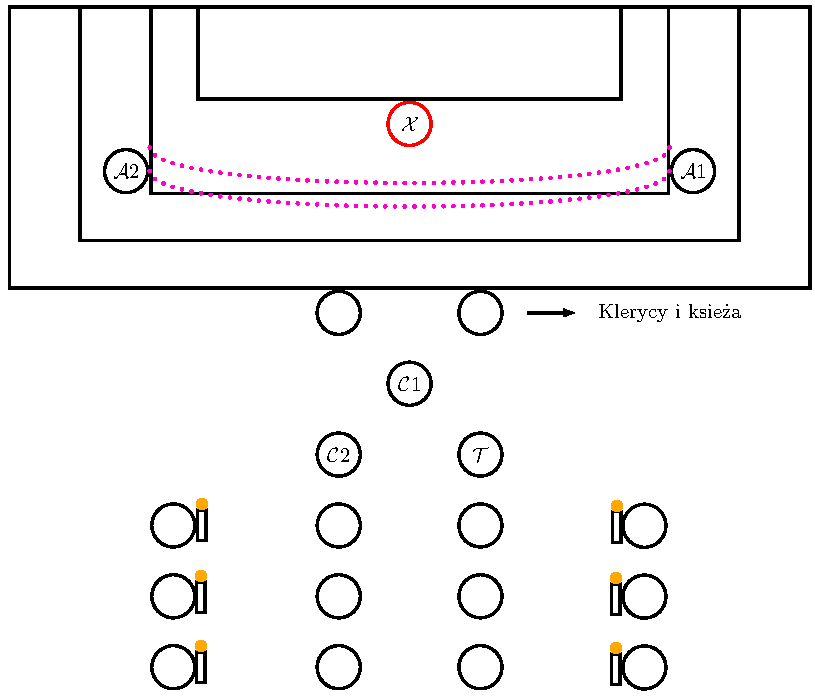
\includegraphics[width=0.5\linewidth]{Figures/Czwartek/Komunia1.pdf}
                  \caption{Przyjmowanie Komunii Św. -- część 1}
            \end{figure}
      \item Przed nimi do kolejki wchodzą księża, klerycy i ceremoniarze, za nimi
            reszta ministrantów z chóru.
      \item \cc1 podaje patenę pierwszemu duchownemu przyjmującemu Komunię św.,
            albo, jeśli nie ma duchownych trzyma ją sam. Po przyjęciu Komunii Św.
            zajmuje miejsce przy \ii, gdzie asystuje z pateną.
      \item \cc2 po przyjęciu Komunii św. zajmuje miejsce przy celebransie ze
            świeczką sanctusową.
      \item \aa\aa~ trzymający obrus przyjmują Komunię św. razem po \cc.
            \begin{figure}[h!]
                  \centering
                  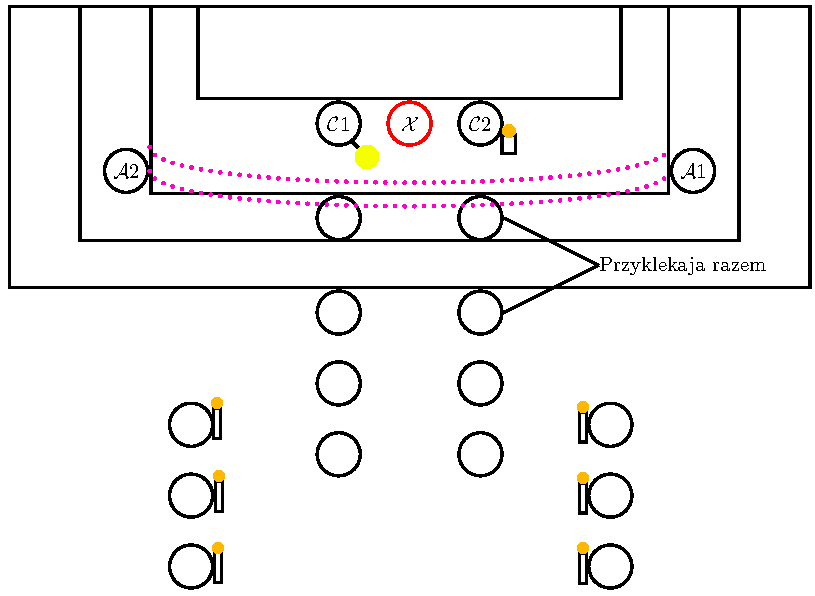
\includegraphics[width=0.5\linewidth]{Figures/Czwartek/Komunia2.pdf}
                  \caption{Przyjmowanie Komunii Św. -- część 2}
            \end{figure}
      \item Każda dwójka przystępująca do Komunii św. przyklęka jednocześnie z
            poprzedzającą parą, wchodzi na stopnie i klęka na dwa kolana. Po
            przyjęciu komunii znów przyklęka jednocześnie z parą stojącą za nimi.
            Ze stopni ołtarza schodzimy w lewo po stopniu diakońskim – do chóru.
      \item Po przyjęciu komunii zapala się znów świece, które trzymają aż do
            procesji do ciemnicy.
      \item Po komunii cały chór klęczy do słów \textit{Dominus vobiscum} z
            zapalonymi już świecami.
      \item \cc3 i \cc4 kierują porządkiem przyjmowania Komunii przez wiernych
            dbając o sprawne przystępowanie i odchodzenie
            \begin{figure}[h!]
                  \centering
                  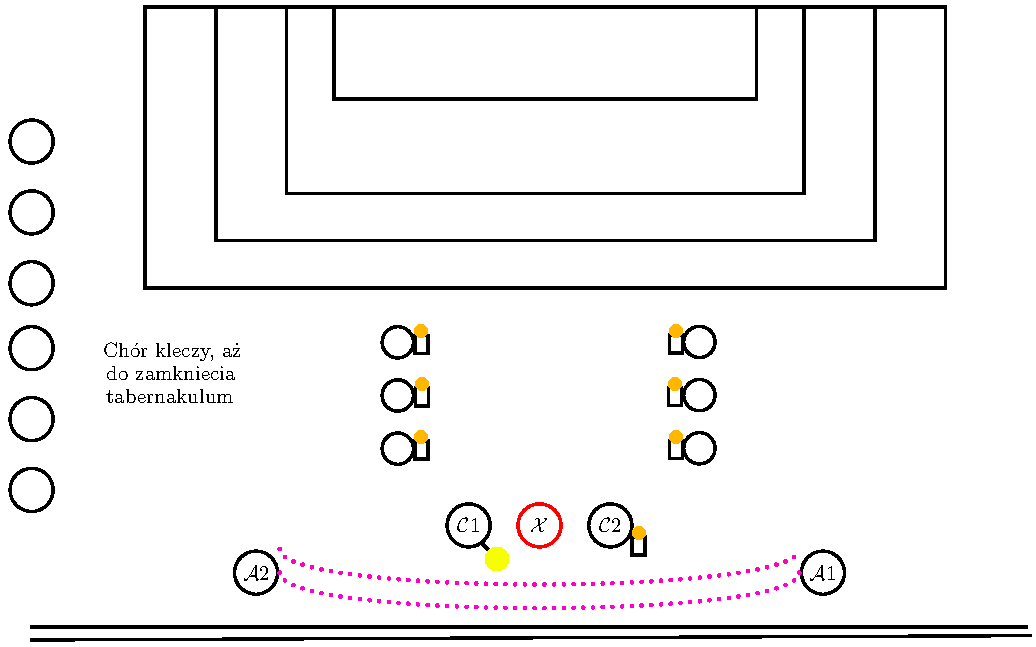
\includegraphics[width=0.5\linewidth]{Figures/Czwartek/Komunia3.pdf}
                  \caption{Przyjmowanie Komunii Św. -- część 3}
            \end{figure}
      \item Do ołtarza \aa\aa~ podchodzą bokiem, przyklękając raz na dole. Do
            przeniesienia mszału i welonu nie idą na skos, ale również bokiem. W
            czasie zabierania welonu i przenoszenia mszału \aa2 zabiera ze sobą
            białe rękawiczki do zniesienia kielicha.
\end{itemize}

\subsection{Zakończenie Mszy}

\begin{itemize}
      \item  Msza święta kończy się słowami \textit{Benedicamus Domino}, następnie
            \ii~ odmawia \textit{Placeat} i całuje ołtarz.
      \item Opuszcza się błogosławieństwo oraz ostatnią ewangelię.
\end{itemize}



\section{Msza Święta - ważniejsze zmiany}
\begin{itemize}
	\item wszyscy odkładają palmy
	\item nie odmawia się modlitw u stopni
	\item bezpośrednio po przyklęknięciu następuje ucałowanie ołtarza i
	      nałożenie kadzidła
	\item po odmówieniu \textit{Introitu} i \textit{Kyrie} \ii~ i \dd~ oraz \ss~
	      krótką drogą schodzą do sedilii
	\item \ii~ (cały czas w asyście \dd) po przeczytaniu lekcji (podczas której
	      nie przyklęka) czyta dalsze propria \footnote{\textit{Graduał} i
		      \textit{Traktus}}. Przyklęka ze wszystkimi, wtedy gdy \ss~ zaśpiewa
	      \textit{\dots in nomine Iesu omne genu flectatur \dots}. Jeżeli do
	      czasu błogosławieństwa \ss~ nie przeczyta wszystkiego, robi przerwę na
	      pobłogosławienie. Siada dopiero po przeczytaniu wszystkiego do
	      Ewangelii wyłącznie lub po błogosławieństwie \ss.
	\item chór śpiewa pełną wersję \textit{Gradułału} melodią standardową oraz
	      \textit{Traktusa} melodią psalmową
	\item procesja przed Ewangelią -- patrz \textit{\nameref{sec:dodatek_palm}}
	\item chór podczas Ewangelii:

	      \begin{itemize}
		      \item trzyma w rękach palmy
		      \item wykonuje skłony przed siebie
		      \item śpiewacy wykonują skłony przed siebie
		      \item klękamy tak jak stoimy przed siebie
	      \end{itemize}

	\item po przyjęciu przez \ii~ Komunii Św. \dd~ śpiewa trzeci confiteor 
	\item nie ma ostatniej Ewangelii
	\item antyfonę \textit{Ave Regina Caelorum} zastępuje się sekwencją
	      \textit{Stabat Mater} na melodię Watykańską.

\end{itemize}

\section{Msza Święta}

\begin{itemize*}
      \item Po modlitwie, \ii~ przebiera się przy sedilli w ornat i zakłada
            manipularz. Jeśli msza jest solenna, \dd~ (i \ss) ubiera(ją)
            manipularz(e). Dalej msza toczy się jak zwykle, z następującymi
            wyjątkami i wskazaniami:
            \begin{itemize*}
                  \item Odmawiamy całe modlitwy u stopni ołtarza.
                  \item Na mszy solennej \ii~ odczytuje lekcję i ewangelię
                  cicho.
                  \item W trakcie śpiewu traktusu na słowa \textit{Adiuva nos,
                        Deus salutaris noster} klękamy.
                  \item Uwaga! \ii~ nie przyklęka podczas odczytywania
                        traktusu --  robi to razem ze wszystkimi podczas śpiewu
                        scholi, na środku na pierwszym stopniu.
                  \item Po modlitwie po komunii jest modlitwa nad ludem. W mszy
                        solennej \dd, po \textit{Oremus} \ii~, obraca się do ludu
                        i śpiewa \textit{Humiliate capita vestra Deo}.
                  \item Na koniec zamiast \textit{Ite, missa est} śpiewa się
                        \textit{Benedicamus Domino} przodem do ołtarza.
                  \item Ważne: Chór klęczy na oba kolana:
                        \begin{itemize*}
                              \item podczas kolekty,
                              \item od \textit{Sanctus} do \textit{Pax Domini},
                              \item podczas modlitwy po komunii i modlitwy nad
                              ludem.
                        \end{itemize*}

            \end{itemize*}

\end{itemize*}

\section{Komunia Święta \textit{bardziej uroczysta}}

\subsection{Komunia Święta dwójkami – bez obrusu komunijnego}

\begin{itemize}
	\item Ministranci biorący udział w lucenarium wchodzą dwójkami do
	      prezbiterium, tworząc w ten sposób naturalną „kolejkę”. Przed nimi do
	      kolejki wchodzą \aa\aa~, trzymając w rękach patenę. Za nimi miejsce
	      zajmuje \cc~ razem z \tt~ lub innym ministrantem.
	\item Na znak \cc cała procesja komunijna najpierw przyklęka, a potem klęka
	      na dwa kolana. \aa\aa~ wchodzą na najwyższy stopień ołtarza i
	      przyjmują Komunię Świętą jako pierwsi.
	\item \aa\aa~ po przyjęciu Komunii Świętej na najwyższym stopniu ołtarza i
	      przyklęknięciu zajmują miejsce przy celebransie z pateną i świeczką
	      sanctusową.
	\item Każda para tuż przed przyjęciem Komunii Świętej przyklęka na podłodze,
	      razem z parą poprzedzającą, która już Komunię przyjęła.
	\item Każda para po przyjęciu Komunii Świętej przyklęka, po czym odchodzi na
	      stronę Ewangelii, w kierunku chóru.
\end{itemize}

\subsection{Śpiewana bardziej uroczysta – z obrusem komunijnym}

\begin{itemize}
	\item Podczas śpiewu \textit{Agnus Dei} \aa1 bierze z kredencji obrus
	      komunijny, razem z \aa2 klękają pośrodku, wchodzą na najwyższy stopień
	      ołtarza i klęcząc przodem do siebie trzymają rozłożony obrus (Rys.
	      \ref{fig:komunia_1}).

	      \begin{figure}[h]
		      \centering
		      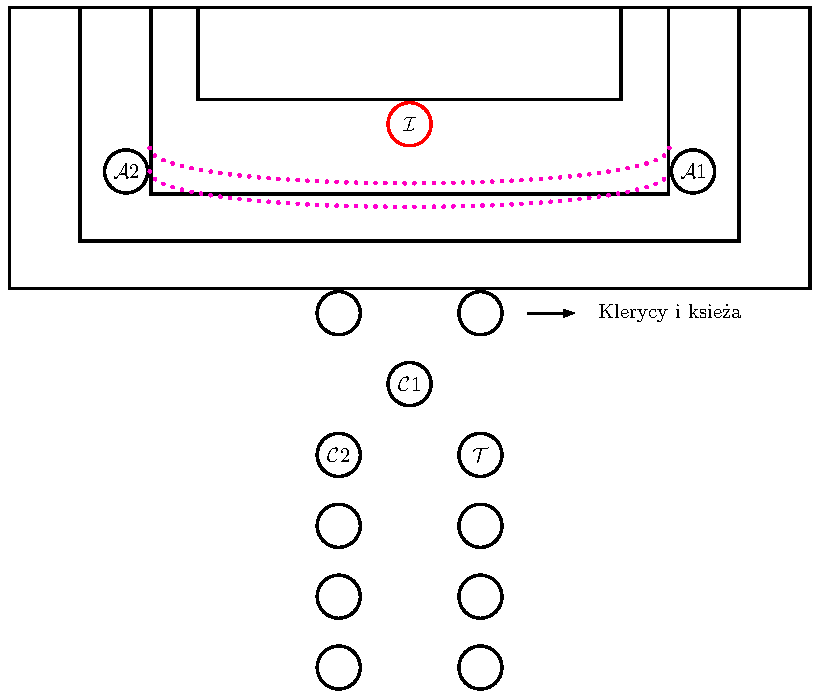
\includegraphics[width=0.5\linewidth]{komunia_1}
		      \caption{Procesja do Komunii Św.}
		      \label{fig:komunia_1}
	      \end{figure}

	\item Ministranci biorący udział w lucenarium wchodzą dwójkami do
	      prezbiterium, tworząc w ten sposób naturalną „kolejkę” do Komunii św.
	      Przed nimi do kolejki wchodzą księża, klerycy i \cc~, za nimi reszta
	      ministrantów z chóru. \cc1 – zależnie od ilości duchownych i
	      ministrantów może staje do komunii sam lub w parze.
	\item \cc~ podaje patenę pierwszemu duchownemu przyjmującemu Komunię św.,
	      albo jeśli nie ma duchownych trzyma ją sam. Po przyjęciu Komunii Św.
	      zajmuje miejsce przy \ii, gdzie asystuje z pateną.
	\item \cc2 lub \tt~ po przyjęciu Komunii św. zajmuje miejsce przy \ii~ ze
	      świeczką sanctusową (Rys. \ref{fig:komunia_2}).

	      \begin{figure}[h]
		      \centering
		      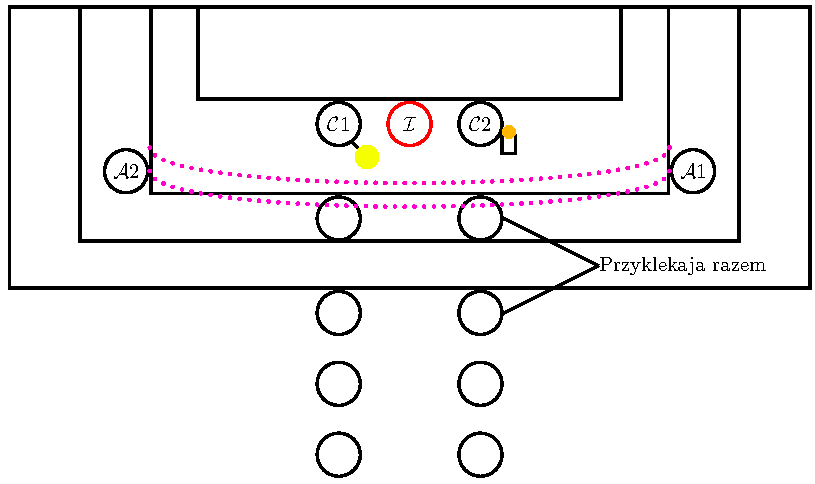
\includegraphics[width=0.5\linewidth]{komunia_2}
		      \caption{W trakcie udzielania Komunii Św. ministrantom}
		      \label{fig:komunia_2}
	      \end{figure}

	\item \aa\aa~ trzymający obrus przyjmują Komunię św. razem z \cc1.
	\item Każda dwójka przystępująca do Komunii św. przyklęka jednocześnie z
	      poprzedzającą parą, wchodzi na stopnie i klęka na dwa kolana. Po
	      przyjęciu komunii znów przyklęka jednocześnie z parą stojącą za nimi.
	      Ze stopni ołtarza schodzimy w lewo – do chóru.
	\item Po przyjęciu Komunii Św. przez ministrantów \aa\aa~ wstają i
	      przechodzą do miejsca udzielania komunii wiernym. Z pateną i świeczką
	      sanctusową asystują \cc\cc~ (Rys. \ref{fig:komunia_3}).

	      \begin{figure}[h]
		      \centering
		      \includegraphics[width=0.5\linewidth]{komunia_3}
		      \caption{W trakcie udzielania Komunii Św. ludowi}
		      \label{fig:komunia_3}
	      \end{figure}

\end{itemize}

\clearpage

\subsection{Msza solenna -- bez obrusu komunijnego}

\begin{itemize}
	\item Podczas śpiewu \textit{Agnus Dei} przekazywany jest znak pokoju – \ss~
	      przekazuje go duchownym w chórze i \cc\cc.
	\item Ministranci biorący udział w lucenarium wchodzą dwójkami do
	      prezbiterium, tworząc w ten sposób naturalną „kolejkę” do Komunii św.
	      Zostawiają przed sobą miejsce dla duchownych, mających przyjąć
	      Komunię. Za nimi ustawia się reszta ministrantów (Rys.
	      \ref{fig:komunia_1_uro_bez})
	\item Jeśli \dd~ lub inny kapłan rozdaje Komunię św., \cc~ asystuje ze
	      świeczką \ii, a \aa\aa~ z pateną i świeczką asystują \dd~ (Rys.
	      \ref{fig:komunia_3_uro_diak_bez}).

	      \begin{figure}[ht]
		      \centering
		      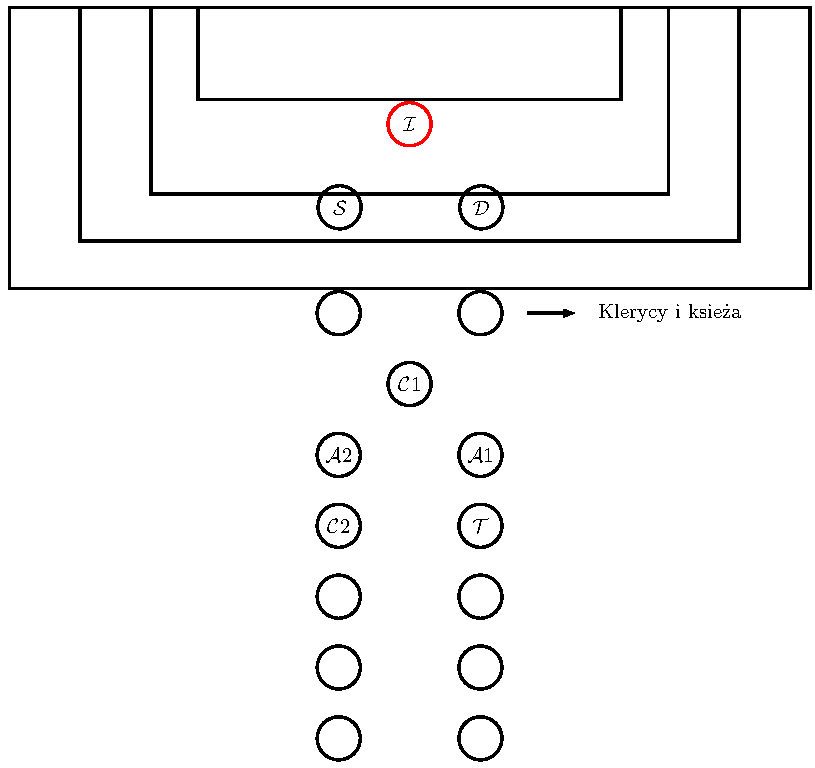
\includegraphics[width=0.5\linewidth]{komunia_1_uro_bez}
		      \caption{W trakcie udzielania Komunii Św. ludowi (diakon rozdaje)}
		      \label{fig:komunia_1_uro_bez}
	      \end{figure}

	      \begin{figure}[ht]
		      \centering
		      \includegraphics[width=0.5\linewidth]{komunia_3_uro_diak_bez}
		      \caption{W trakcie udzielania Komunii Św. ludowi (diakon rozdaje)}
		      \label{fig:komunia_3_uro_diak_bez}
	      \end{figure}
\end{itemize}

\subsection{Msza solenna -- z obrusem komunijnym}

\begin{itemize}
	\item Po ewentualnym. odebraniu znaku pokoju \aa1 bierze z kredencji obrus
	      komunijny, razem z \aa2 klękają pośrodku, wchodzą na najwyższy stopień
	      ołtarza i klęcząc przodem do siebie trzymają rozłożony obrus.
	\item Porządek Komunii Św. (patrz obrazki przy mszy śpiewanej z obrusem)
	      \begin{itemize}
		      \item \dd~ i \ss~
		      \item kapłani, klerycy
		      \item \aa\aa~ trzymający obrus i \cc1
		      \item \cc2 i \tt~
		      \item reszta ministrantów.
	      \end{itemize}
	\item Jeśli \dd~ nie rozdaje komunii, razem z \ss~ asystują \ii. Podąża za
	      nimi \cc1 ze świeczką sanctusową (Rys. \ref{fig:komunia_3_uro}).

	      \begin{figure}[h]
		      \centering
		      \includegraphics[width=0.5\linewidth]{komunia_3_uro}
		      \caption{W trakcie udzielania Komunii Św. ludowi (\dd~ nie rozdaje)}
		      \label{fig:komunia_3_uro}
	      \end{figure}

	\item Jeśli \dd~ lub inny kapłan rozdaje komunię przy obrusie (Rys.
	      \ref{fig:komunia_3_uro_1}):

	      \begin{itemize}
		      \item \ii~ asystuje \ss~ z pateną
		      \item \dd~ asystuje \cc2 z pateną
		      \item dwóch wyznaczonych ministrantów z chóru po przyjęciu Komunii
		            zapala świeczki i przy udzielaniu komunii wiernym, klęczą ze
		            świeczkami po dwóch stronach obrusa.
	      \end{itemize}

	      \begin{figure}[ht]
		      \centering
		      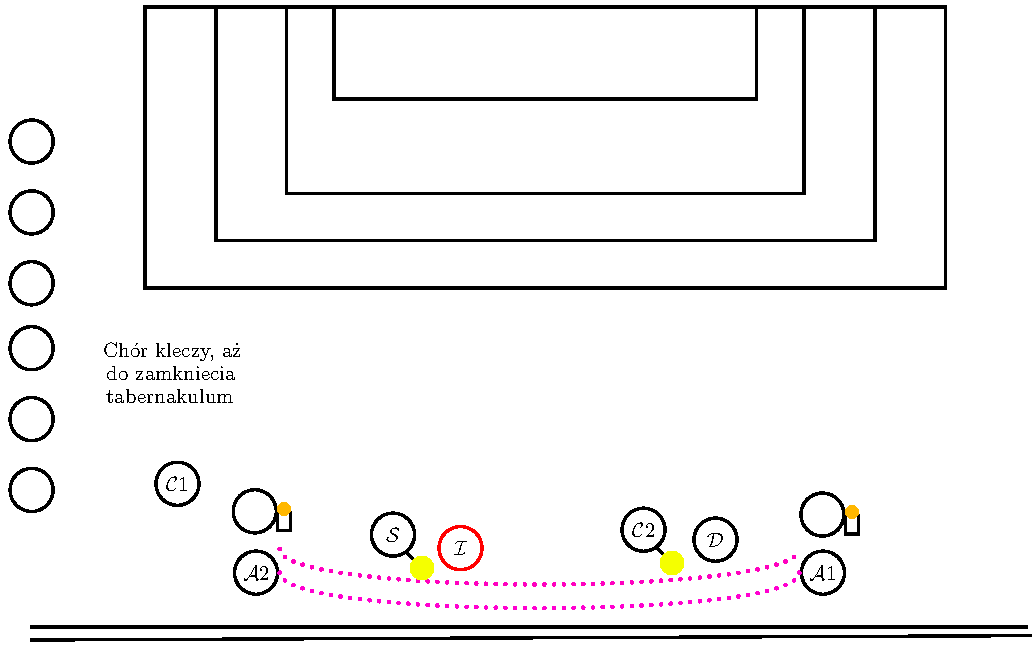
\includegraphics[width=0.5\linewidth]{komunia_3_uro_diak}
		      \caption{W trakcie udzielania Komunii Św. ludowi (\dd~ rozdaje)}
		      \label{fig:komunia_3_uro_1}
	      \end{figure}

\end{itemize}

\clearpage


\end{document}
